\documentclass{book}
   
\usepackage{commeunjeustyle} 

\begin{document}

\chapter*{Exemple fil de rouge de l'algèbre linéaire}

\begin{Texte}
L'algèbre linéaire est un outil essentiel pour toutes les branches des mathématiques, en particulier lorsqu'il s'agit
de modéliser puis résoudre numériquement des problèmes issus de divers domaines : des sciences physiques ou
mécaniques, des sciences du vivant, de la chimie, de l'économie, des sciences de l'ingénieur...\\
Cette exemple introductif permet de présenter les \impo{différentes représentations} de l'objet mathématique système d'équations linéaires.
\end{Texte}
\begin{Exemple}
Problème : la somme des tailles d'un fils et du père est de 2,5 mètres. La différence de tailles  est de 0.5 mètres.
Quelle est la taille du fils et du père ? \\
\impo{Modélisation : }\\  
Soit l'inconnue $x$ représentant la taille du fils et l'inconnue $y$ représentant la taille du père.\\
La somme est 2,5 donc $x+y=2,5$.\\
La différence est 0,5 donc $y-x=0,5$.\\
Ainsi on cherche $x$ et $y$ vérifiant le système $(S)$  :
\begin{center}
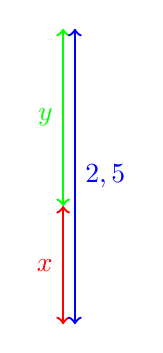
\begin{tikzpicture}[scale=1.5]
\draw[line width=0.3mm, <->,color=red] (0,0) -- node[left] {$x$}(0,1);
\draw[line width=0.3mm, <->,color=green] (0,1) -- node[left] {$y$}(0,2.5);
\draw[line width=0.3mm, <->,color=blue] (0.1,0) -- node[right] {$2,5$}(0.1,2.5);
\end{tikzpicture}
et
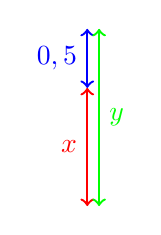
\begin{tikzpicture}[scale=1.5]
\draw[line width=0.3mm, <->,color=red] (0,0) -- node[left] {$x$}(0,1);
\draw[line width=0.3mm, <->,color=blue] (0,1) -- node[left] {$0,5$}(0,1.5);
\draw[line width=0.3mm, <->,color=green] (0.1,0) -- node[right] {$y$}(0.1,1.5);
\end{tikzpicture}
$\Leftrightarrow\quad \begin{cases}
{\color{red}x}+{\color{green}y}&={\color{blue}2,5}\\
{\color{red}x}+{\color{blue}0,5}&={\color{green}y}
\end{cases}\Leftrightarrow\quad \begin{cases}
{\color{red}x}+{\color{green}y}&={\color{blue}2,5}\\
{\color{red}-x}+{\color{green}y}&={\color{blue}0,5}
\end{cases}
$		
\end{center}
\end{Exemple}
\section{Système d'équations}

\subsection{Résolution algébrique}
Pour déterminer l'ensemble des solutions $x$ et $y$ vérifiant ce système, une idée est de découpler par itérations les dépendances entre les inconnues dans les équations par combinaison ou élimination. A chaque itération, ces deux opérations transforment  un système d'équations en un autre équivalent (ayant les mêmes solutions).\\
L'application à l'exemple introductif est :
\begin{enumerate}
\item pour éliminer $x$ de la ligne 2,  on ajoute à la ligne 2 la ligne 1 :
$$\begin{cases}
x+y&=2,5\\
2y&=3
\end{cases}
$$
\item pour déterminer $y$, on divise la ligne 2 par 2 : 
$$\begin{cases}
x+y&=2,5\\
y&=1,5
\end{cases}
$$
\item pour éliminer $y$  de la ligne 2, on soustraie à la ligne 1 la ligne 2 :
$$\begin{cases}
x&=1\\
y&=1,5
\end{cases}
$$
\end{enumerate}
Ainsi l'ensemble des solution est l'unique solution $(1 , 1,5 )$ car ce dernier système d'équations est équivalent au premier.\\
Cette approche sera l'objet du chapitre système d'équations linéaires. 
\subsection{Résolution géométrique}
Le système équation :
$$(S)\quad \begin{cases}
x+y&=2,5\quad(D_1)\\
-x+y&=0,5\quad(D_2)
\end{cases}$$
est constitué de deux équations de deux droites $D_1$ et $D_2$.\\
Trois cas se présentent alors :
\begin{enumerate}
\item Si les droites $D_1$ et $D_2$ ne sont pas parallèles, alors elle s'intersecte en un unique point et le système $(S)$ a une
unique solution.
\begin{center}
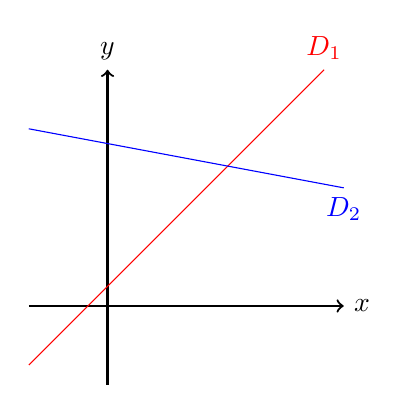
\begin{tikzpicture}[scale=0.5]
\draw[thick,->] (-2,0) -- (6,0)node[anchor=west] {$x$};
\draw[thick,->] (0,-2) -- (0,6)node[anchor=south] {$y$};
\draw[-,color=red] (-2,-1.5) -- (5.5,6)node[anchor=south] {$D_1$};
\draw[-,color=blue] (-2,4.5) -- (6,3)node[anchor=north] {$D_2$};
\end{tikzpicture}	
\end{center}
\item Si les droites $D_1$ et $D_2$  sont parallèles et non confondues, alors elle ne s'intersecte pas et le système $(S)$ n'a pas de solution.
\begin{center}
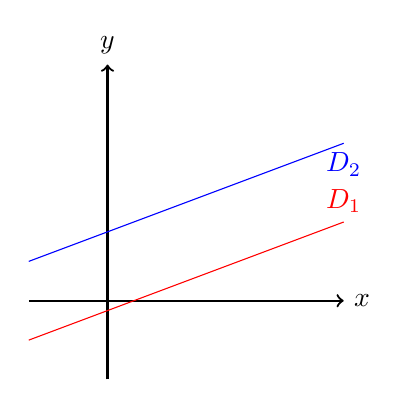
\begin{tikzpicture}[scale=0.5]
\draw[thick,->] (-2,0) -- (6,0)node[anchor=west] {$x$};
\draw[thick,->] (0,-2) -- (0,6)node[anchor=south] {$y$};
\draw[-,color=red] (-2,-1) -- (6,2)node[anchor=south] {$D_1$};
\draw[-,color=blue] (-2,1) -- (6,4)node[anchor=north] {$D_2$};
\end{tikzpicture}	
\end{center}
\item Si les droites $D_1$ et $D_2$  sont parallèles et  confondues, alors elle s'intersecte en une infinité de points et le système $(S)$ a une infinité de solutions.
\begin{center}
\begin{tikzpicture}[scale=0.5]
\draw[thick,->] (-2,0) -- (6,0)node[anchor=west] {$x$};
\draw[thick,->] (0,-2) -- (0,6)node[anchor=south] {$y$};
\draw[-,color=red] (-2,-1) -- (6,4)node[anchor=south] {$D_1=D_2$};
\end{tikzpicture}
\end{center}
\end{enumerate} 
%Nous verrons plus loin que ces trois cas de figure (une seule solution, aucune solution, une infinité de solutions) sont
%les seuls cas qui peuvent se présenter pour n'importe quel système d'équations linéaires.\\
Dans notre exemple, comme les vecteurs normaux aux deux droites $\begin{pmatrix}
1\\1
\end{pmatrix}$ et $\begin{pmatrix}
-1\\1
\end{pmatrix}$ ne sont pas colinéaires, les deux droites ne sont pas parallèles et donc admettent un unique point d'intersection.
\begin{center}
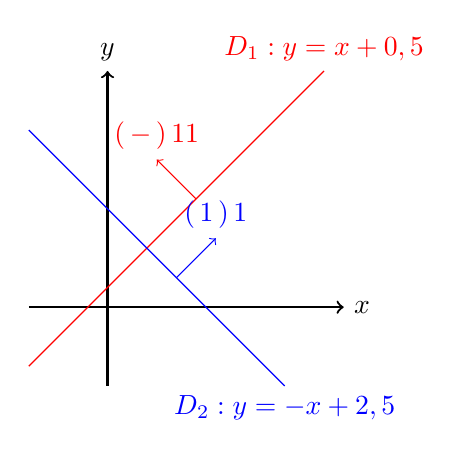
\begin{tikzpicture}[scale=0.5]
%\draw[step=1cm,gray,very thin] (-2,-2) grid (6,6);
\draw[thick,->] (-2,0) -- (6,0)node[anchor=west] {$x$};
\draw[thick,->] (0,-2) -- (0,6)node[anchor=south] {$y$};
%\foreach \x in {-2,-1,0,1,2,3,4,5}
%   \draw (\x cm,1pt) -- (\x cm,-1pt) node[anchor=north] {$\x$};
%\foreach \y in {-2,-1,0,1,2,3,4,5}
%    \draw (1pt,\y cm) -- (-1pt,\y cm) node[anchor=east] {$\y$};
\draw[-,color=red] (-2,-1.5) -- (5.5,6)node[anchor=south] {$D_1 : y=x+0,5$};
\draw[-,color=blue] (-2,4.5) -- (4.5,-2)node[anchor=north] {$D_2 : y=-x+2,5$};

\draw[->,color=red] (2.25,2.75) -- (1.25,3.75)node[anchor=south] {$\begin{pmatrix}-1\\1\end{pmatrix}$};

\draw[->,color=blue] (1.75,0.75) -- (2.75,1.75)node[anchor=south] {$\begin{pmatrix}1\\1\end{pmatrix}$};
\end{tikzpicture}	
\end{center}
Ainsi l'ensemble des solution admet une unique solution. Par lecture graphique, l'unique solution est $(1 , 1,5 )$.
La notion de vecteurs normaux sera l'objet du chapitre \impo{espaces préhilbertiens}. 
\section{Calcul matricielle}
On sait résoudre par de simples opérations algébriques une équation linéaire à une inconnue. Par exemple, pour l'équation $2x+1=5$, on additionne l'opposé de $1$, soit $-1$ $$2x+1+(-1)=5+(-1)$$ ce qui donne $2x=4$, puis on multiple par l'inverse de 2, ce qui donne $x=2$.\\
Une idée est de transformer le système de deux équations à deux inconnues à une équation à une inconnue. Cette transformation est une abstraction sur la nature des coefficients et des variables des équations : de \impo{réels} à  \impo{tableaux de nombres}.\\
Ainsi, l'équation équivalente au système d'équations linéaires est  :
\begin{center}
$\begin{cases}
{\color{red}x}+{\color{green}y}&={\color{blue}2,5}\\
{\color{red}-x}+{\color{green}y}&={\color{blue}0,5}
\end{cases}\Leftrightarrow
$	
\begin{tikzpicture}[scale=1,>=latex]
\matrix (A) [matrix of math nodes,%
             nodes = {circle,minimum size=1cm},%
             left delimiter  = (,%
             right delimiter = )] at (-2.5cm,0)
{%
  1 & 1   \\
 -1 & 1  \\
};
\matrix (B) [matrix of math nodes,%
             nodes = {circle,minimum size=1cm},%
             left delimiter  = (,%
             right delimiter =)] at (0,2.5cm)
{%
  \color{red}x\\
  \color{green}y\\
};
\draw[dotted] (.7cm,0) node {$=$};
\matrix (Y) [matrix of math nodes,%
             nodes = {circle,minimum size=1cm},%
             left delimiter  = (,%
             right delimiter = )] at (2.2cm,0)
{%
  \color{blue}2,5  \\
  \color{blue}0,5 \\
};
\draw[<->,colordef](A-1-1) to[in=180,out=90]
    node[draw,sloped,midway,fill=white] (x) {$1\times x$} (B-1-1);
\draw[<->,colordef](A-1-2) to[in=180,out=90]
    node[draw,sloped,midway,fill=white] (y) {$1\times y$} (B-2-1);
\draw[colordef,->] (x) to node[midway,sloped,fill=white] {$+$} (y);
\end{tikzpicture}
\end{center}
Autrement dit, on $$A\times X =B$$ avec $A=\begin{pmatrix}
 1 & 1   \\
 -1 & 1  \\
\end{pmatrix}, X=\begin{pmatrix}
 x   \\
 y  \\
\end{pmatrix}$ et $B=\begin{pmatrix}
 2,5   \\
 0,5  \\
\end{pmatrix}$.\\
En calculant le déterminant de la matrice (voir chapitre \impo{déterminant)}, on démontre que la matrice  $\begin{pmatrix}
 1 & 1   \\
 -1 & 1  \\
\end{pmatrix}$ est inversible, c'est à dire qu'il existe une matrice $A^{-1}=\begin{pmatrix}
 \frac 1 2 & -\frac 1 2   \\
 \frac 1 2 & \frac 1 2  \\
\end{pmatrix}$  telle que, en multipliant, par $A^{-1}$ les deux membres de l'équation $A\times X =B$, on obtient :
$$ X=A^{-1}B$$
$$ \begin{pmatrix}
 x   \\
 y  \\
\end{pmatrix}=\begin{pmatrix}
 \frac 1 2 & -\frac 1 2   \\
 \frac 1 2 & \frac 1 2  \\
\end{pmatrix} \begin{pmatrix}
 2,5   \\
 0,5  \\
\end{pmatrix}= \begin{pmatrix}
 1  \\
 1,5  \\
\end{pmatrix}.$$ 
Par identification, l'ensemble des solution est de nouveau l'unique solution $x=1$ et $y=1,5$. 
Les\impo{matrices} seront étudiées dans le chapitre \impo{matrices}. 
\section{Espace vectoriel}
Une idée est de transformer ce système de deux équations à deux inconnues en un système d'une équation à deux inconnues. On a :\\
$$\begin{cases}
{\color{red}x}+{\color{green}y}&={\color{blue}2,5}\\
{\color{red}-x}+{\color{green}y}&={\color{blue}0,5}
\end{cases}
\Leftrightarrow
	 {\color{red}x}\begin{pmatrix}
 1    \\
 -1   \\
\end{pmatrix}+{\color{green}y}\begin{pmatrix}
  1   \\
  1  \\
\end{pmatrix}=\begin{pmatrix}
 {\color{blue}2,5}   \\
 {\color{blue}0,5}  \\
\end{pmatrix}$$
Il s'agit de déterminer $x,y$ afin d'exprimer $\begin{pmatrix}
 2,5   \\
 0,5  \\
\end{pmatrix}$  comme une combinaison linéaire de la famille des vecteurs $(\begin{pmatrix}
 1    \\
 -1   \\
\end{pmatrix},\begin{pmatrix}
 1   \\
  1  \\
\end{pmatrix})$. 
\begin{center}
\begin{tikzpicture}[general,scale=1.5]
\draw [quadrillage] (-0.1,-1.1) grid (3,1.1);
\axeX{-0.1}{3}{1}
\axeY{-1.1}{1.1}{1}
\draw [->, epais] (0,0) -- (1,-1)node[right]{$\begin{pmatrix}
 1    \\
 -1   \\
\end{pmatrix}$};
\draw [->, epais] (0,0) -- (1,1)node[right]{$\begin{pmatrix}
 1    \\
 1   \\
\end{pmatrix}$};
\draw [->, epais] (0,0) -- (2.5,0.5)node[right]{$\begin{pmatrix}
 {\color{blue}2,5}   \\
 {\color{blue}0,5}  \\
\end{pmatrix}$};
\draw [->, epais] (0,0) -- (2.3,-0.5)node[right]{$ {\color{red}x}\begin{pmatrix}
 1    \\
 -1   \\
\end{pmatrix}+{\color{green}y}\begin{pmatrix}
  1   \\
  1  \\
\end{pmatrix}$};
\end{tikzpicture}
\end{center}
Avec GeoGebra \url{https://www.geogebra.org/m/shsawcqc}), on trouve l'unique couple $(x=1,y=1,5)$. D'un point de vue mathématiques, on se pose trois questions :
\begin{enumerate}
\item \impo{Existence:} la famille est-elle \impo{génératrice} de $\R^2$ ? C'est à dire, peut-on  exprimer tout vecteur de $\R^2$ comme  une combinaison linéaire de la famille des vecteurs $(\begin{pmatrix}
 1    \\
 -1   \\
\end{pmatrix},\begin{pmatrix}
 1   \\
  1  \\
\end{pmatrix})$ ? Si cela est vraie, alors, en particulier,  le vecteur $\begin{pmatrix}
 2,5   \\
 0,5  \\
\end{pmatrix}$ s'exprime comme  une combinaison linéaire de la famille des vecteurs $(\begin{pmatrix}
 1    \\
 -1   \\
\end{pmatrix},\begin{pmatrix}
 1   \\
  1  \\
\end{pmatrix})$.
\item \impo{Unicité:} la famille est-elle \impo{libre} ? Lorsque un vecteur de $\R^2$ s'exprime comme combinaison linéaire de   $\begin{pmatrix}
 1    \\
 -1   \\
\end{pmatrix}$ et $\begin{pmatrix}
 1   \\
  1  \\
\end{pmatrix}$, y-a-il unicité de cette combinaison  linéaire ? Si cela est vraie, alors, en particulier, il y a unicité  de la combinaison linéaire pour exprimer le vecteur $\begin{pmatrix}
 2,5   \\
 0,5  \\
\end{pmatrix}$.
\item \impo{Existence} et \impo{Unicité} : la famille est-elle \impo{base} ? c'est à dire la famille est-elle \impo{génératrice et libre} ? c'est à dire peut-on  exprimer tout vecteur de $\R^2$ comme  une unique combinaison linéaire de la famille des vecteurs $(\begin{pmatrix}
 1    \\
 -1   \\
\end{pmatrix},\begin{pmatrix}
 1   \\
  1  \\
\end{pmatrix})$ ?. Si cela est vraie, alors, en particulier, il y a existence et unicité  de la combinaison linéaire pour exprimer le vecteur $\begin{pmatrix}
 2,5   \\
 0,5  \\
\end{pmatrix}$ et l'ensemble des solutions est un unique couple.  
\end{enumerate}
L'étude des combinaisons linéaires sera fait dans le chapitre sur les espaces vectoriels. 
\section{Application linéaire}
La dernière idée est de considérer le membre de gauche de l'équation comme l'image d'une fonction :
\begin{center}
$
\begin{cases}
{\color{red}x}+{\color{green}y}&={\color{blue}2,5}\\
{\color{red}-x}+{\color{green}y}&={\color{blue}0,5}
\end{cases}
\Leftrightarrow\quad \begin{pmatrix}
 {\color{red}x} +{\color{green}y}   \\
 {\color{red}-x} +{\color{green}y}   \\
\end{pmatrix} =\begin{pmatrix}
 {\color{blue}2,5}   \\
 {\color{blue}0,5}  \\
\end{pmatrix}
\Leftrightarrow\quad
u(\begin{pmatrix}
 \color{red}x     \\ {\color{green}y}   \\
\end{pmatrix})
	 = \begin{pmatrix}
 {\color{blue}2,5}   \\
 {\color{blue}0,5}  \\
\end{pmatrix}$\\
\begin{tikzpicture}[general,scale=1]
\draw [->, epais] (0,0)node[left]{avec $\quad \begin{pmatrix}
 {\color{red}x}    \\
{\color{green}y}   \\
\end{pmatrix}$} -- (1,0);
\draw [-, epais] (1,-1)--(2.5,-1)--(2.5,1)--(1,1)--(1,-1);
\draw(1.75,0) node{$u$};
\draw [->, epais] (2.5,0) -- (3.5,0)node[right]{$\begin{pmatrix}
 {\color{red}x} + {\color{green}y}    \\
 {\color{red}-x}+  {\color{green}y}   \\
\end{pmatrix}$};
\end{tikzpicture} 
\end{center}
Les solutions du système sont l'ensemble des antécédents $\begin{pmatrix}
 {\color{blue}2,5}   \\
 {\color{blue}0,5}  \\
\end{pmatrix}$ par la fonction à deux variables $\Fonction{u}{\R^2}{\R^2}{\begin{pmatrix}
  {\color{red}x}    \\
 {\color{green}y}   \\
\end{pmatrix}}{\begin{pmatrix}
  {\color{red}x} +{\color{green}y}   \\
  {\color{red}-x} +{\color{green}y}   \\
\end{pmatrix}}$.\\
L'étude générale des fonctions à plusieurs variables est compliquée et est fait dans un cours d'analyse,  
cependant,  du fait que la fonction $u$ possède une propriété de linéarité:
 $$u(\begin{pmatrix}
 {x}    \\
{y}   \\
\end{pmatrix}+\begin{pmatrix}
 {x'}    \\
{y'}   \\
\end{pmatrix})=u(\begin{pmatrix}
 {x}    \\
{y}   \\
\end{pmatrix})+u(\begin{pmatrix}
 {x'}    \\
{y'}   \\
\end{pmatrix}) \quad\text{ et }\quad u(\lambda \begin{pmatrix}
 {x}    \\
{y}   \\
\end{pmatrix})=\lambda u(\begin{pmatrix}
 {x}    \\
{y}   \\
\end{pmatrix})$$
son étude est plus facile. Ainsi on peut démontrer qu'elle est bijective et que donc il existe une unique vecteur antécédent au vecteur $\begin{pmatrix}
 {\color{blue}2,5}   \\
 {\color{blue}0,5}  \\
\end{pmatrix}$. Le système admet une unique solution.\\
L'étude des applications linéaires sera fait dans le chapitre \impo{applications linéaires}.




%Système linéaire
%matrices
%espace vectoriel
%application linéaires
%matrices et applications linéaires
%determinant
%categories d'applications linéaires
%polynome d'endomrophismes
%reduction
%espace prehilbertion
%endomorphismes remarquables d’un espace euclidien


\end{document}
